\documentclass{article}
\usepackage{graphicx}
\usepackage[margin=1.5cm]{geometry}
\usepackage{amsmath}

\begin{document}

\title{Wednesday Reading Assessment: Unit 8, Momentum}
\author{Prof. Jordan C. Hanson}

\maketitle

\section{Memory Bank}

\begin{itemize}
\item $\vec{p} = m\vec{v}$ ... Definition of momentum.
\item $\vec{p}_{\rm 1,i} + \vec{p}_{\rm 2,i} = \vec{p}_{\rm 1,f} + \vec{p}_{\rm 2,f}$ ... Momentum conservation for two objects interacting.
\end{itemize}

\section{Momentum}

\begin{enumerate}
\item
\begin{figure}[ht]
\centering
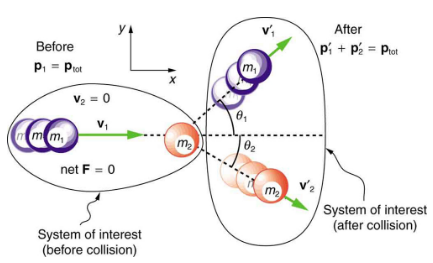
\includegraphics[width=0.4\textwidth]{collision2.png}
\caption{\label{fig:collision} A particle interacts with one at rest.}
\end{figure}
Suppose a mass $m_1$ approaches another mass $m_2$ with velocity $v_{\rm 1,i}$, while $m_2$ is at rest.  Apply momentum conservation to show that, in the x-coordinate,
\begin{equation}
m_1 v_{1,i} = m_1 v_{1,f}\cos\theta_1 + m_2 v_{2,f}\cos\theta_2
\end{equation} \\ \vspace{1cm}
\item Similarly, show that, in the y-coordinate,
\begin{equation}
0 = m_1 v_{1,f}\sin\theta_1 + m_2 v_{2,f}\sin\theta_2
\end{equation} \\ \vspace{1cm}
\item Let $m_1 = 0.1$ kg, and $m_2 = 0.05$ kg.  Also, $\theta_1$ is observed to be 25 degrees, and $\theta_2$ is observed to be 50 degrees.  If $v_{\rm 1,f} = 1.0$ m/s, what is $v_{\rm 2,f}$?
\end{enumerate}
\end{document}
